
\documentclass[border=5pt]{standalone}
\usepackage{tikz}
\usetikzlibrary{arrows.meta, backgrounds, decorations.pathreplacing,
                 fit, shapes.geometric}
\usepackage{amsmath, amssymb}
\usepackage{bm}

\definecolor{colglobal}{HTML}{4F6D7A}
\definecolor{colpop}{HTML}{8F5A83}
\definecolor{coldet}{HTML}{1F9D8A}
\definecolor{colsample}{HTML}{8A4F7D}
\definecolor{coldata}{HTML}{D8D8D8}

\tikzset{
    dag node/.style={
        draw=black!70, semithick, align=center,
        font=\footnotesize, inner sep=2.3pt,
    },
    global/.style={dag node, rectangle, rounded corners=2pt,
        minimum width=1.45cm, minimum height=0.56cm, fill=colglobal!10},
    input/.style={dag node, rectangle, rounded corners=2pt,
        dashed, draw=black!60, minimum width=1.45cm,
        minimum height=0.56cm, fill=coldata!35},
    selection/.style={dag node, rectangle, dashed, draw=black!60,
        fill=white, minimum width=1.85cm, minimum height=0.56cm},
    popdist/.style={dag node, rectangle, draw=colpop!85!black,
        dashed, fill=colpop!8, minimum height=0.66cm,
        text width=1.95cm, inner sep=1.3pt},
    latent/.style={dag node, ellipse, fill=white,
        minimum width=1.45cm, minimum height=0.58cm},
    det/.style={dag node, diamond, aspect=2.35, draw=coldet!85!black,
        fill=coldet!8, inner xsep=1pt, inner ysep=1pt},
    sample/.style={dag node, rectangle, draw=colsample!85!black,
        fill=colsample!8, minimum height=0.62cm,
        text width=1.95cm, inner sep=1.3pt},
    data/.style={dag node, rectangle, very thick, fill=coldata,
        minimum width=1.5cm, minimum height=0.56cm},
    conditioned/.style={data, double, double distance=1pt},
    plate/.style={draw=black!55, rounded corners=5pt, dashed,
        inner xsep=9pt, inner ysep=10pt},
    level label/.style={font=\scriptsize, text=black!70},
    dag edge/.style={-{Stealth[length=3pt, width=2.5pt]}, thin,
        draw=black!55},
    sel edge/.style={dag edge, draw=black!38},
}

\begin{document}
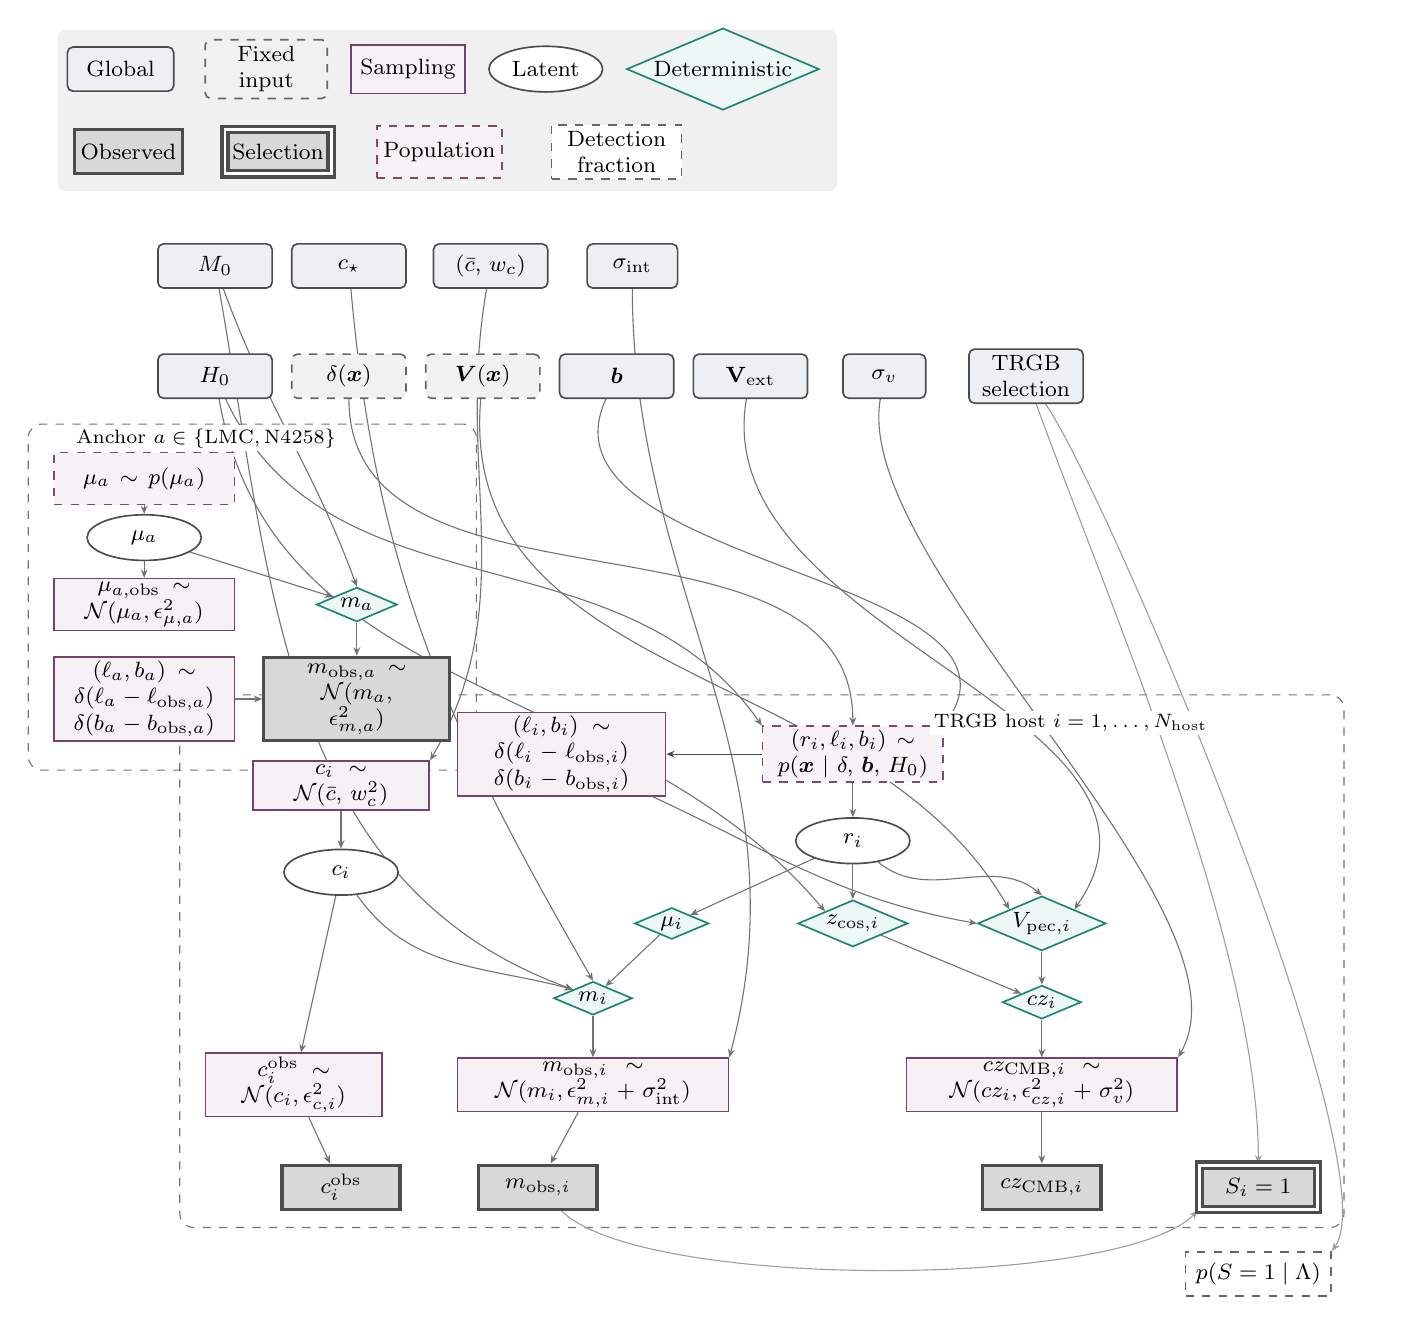
\begin{tikzpicture}

% No manual bounding box: standalone crops to the ink, so the figure is not
% padded with dead margin that \includegraphics would then scale away.

% ===== LEGEND =====
\begin{scope}[on background layer]
    \fill[black!6, rounded corners=3pt] (-1.35, 10.70)
        rectangle (8.55, 12.75);
\end{scope}
\node[global, minimum width=1.35cm] at (-0.55, 12.25) {Global};
\node[input, minimum width=1.55cm] at (1.30, 12.25) {Fixed\\input};
\node[sample, text width=1.35cm] at (3.10, 12.25) {Sampling};
\node[latent, minimum width=1.25cm] at (4.85, 12.25) {Latent};
\node[det, minimum width=1.25cm] at (7.10, 12.25) {Deterministic};
\node[data, minimum width=1.35cm] at (-0.45, 11.20) {Observed};
\node[conditioned, minimum width=1.35cm] at (1.45, 11.20) {Selection};
\node[popdist, text width=1.50cm] at (3.50, 11.20) {Population};
\node[selection, minimum width=1.65cm] at (5.75, 11.20)
    {Detection\\fraction};

% ===== NODES =====
\node[global] (Mtrgb) at (0.65, 9.75) {$M_0$};
\node[global] (cstar) at (2.35, 9.75) {$c_\star$};
\node[global] (cpars) at (4.15, 9.75) {$(\bar c,\,w_c)$};
\node[global, minimum width=1.15cm] (sigint) at (5.95, 9.75) {$\sigma_{\rm int}$};
\node[global] (H0) at (0.65, 8.35) {$H_0$};
\node[input] (rho) at (2.35, 8.35) {$\delta(\bm{x})$};
\node[input] (Vfield) at (4.05, 8.35) {$\bm{V}(\bm{x})$};
\node[global] (bias) at (5.75, 8.35) {$\bm{b}$};
\node[global] (pv) at (7.45, 8.35) {$\mathbf{V}_{\rm ext}$};
\node[global, minimum width=1.05cm] (sigv) at (9.15, 8.35) {$\sigma_v$};
\node[global] (selcuts) at (10.95, 8.35) {TRGB\\selection};
\node[popdist, text width=2.20cm] (anchprior) at (-0.25, 7.05) {$\mu_a \sim p(\mu_a)$};
\node[latent] (anchmu) at (-0.25, 6.30) {$\mu_a$};
\node[sample, text width=2.20cm] (anchgeom) at (-0.25, 5.45) {$\mu_{a,\rm obs} \sim$\\$\mathcal{N}(\mu_a,\epsilon_{\mu,a}^2)$};
\node[det] (anchmtrue) at (2.45, 5.45) {$m_a$};
\node[sample, text width=2.20cm] (anchsky) at (-0.25, 4.25) {$(\ell_a,b_a) \sim$\\$\delta(\ell_a-\ell_{{\rm obs},a})$\\$\delta(b_a-b_{{\rm obs},a})$};
\node[data, text width=2.20cm] (anchmobs) at (2.45, 4.25) {$m_{{\rm obs},a} \sim$\\$\mathcal{N}(m_a,$\\$\epsilon_{m,a}^2)$};
\node[sample, text width=2.55cm] (skydelta) at (5.05, 3.55) {$(\ell_i,b_i) \sim$\\$\delta(\ell_i-\ell_{{\rm obs},i})$\\$\delta(b_i-b_{{\rm obs},i})$};
\node[popdist, text width=2.20cm] (rdist) at (8.75, 3.55) {$(r_i,\ell_i,b_i) \sim$\\$p(\bm{x}\mid\delta,\,\bm{b},\,H_0)$};
\node[latent] (rtrue) at (8.75, 2.45) {$r_i$};
\node[det] (mu) at (6.45, 1.40) {$\mu_i$};
\node[det] (zcos) at (8.75, 1.40) {$z_{{\rm cos},i}$};
\node[det] (vpec) at (11.15, 1.40) {$V_{{\rm pec},i}$};
\node[sample, text width=2.15cm] (cdist) at (2.25, 3.15) {$c_i \sim$\\$\mathcal{N}(\bar c,\,w_c^2)$};
\node[latent] (ctrue) at (2.25, 2.05) {$c_i$};
\node[sample, text width=2.15cm] (csamp) at (1.65, -0.65) {$c_i^{\rm obs} \sim$\\$\mathcal{N}(c_i,\epsilon_{c,i}^2)$};
\node[data] (cobs) at (2.25, -1.95) {$c_i^{\rm obs}$};
\node[det] (mtrue) at (5.45, 0.45) {$m_i$};
\node[det] (cztrue) at (11.15, 0.40) {$cz_i$};
\node[sample, text width=3.35cm] (msamp) at (5.45, -0.65) {$m_{{\rm obs},i} \sim$\\$\mathcal{N}(m_i,\epsilon_{m,i}^2+\sigma_{\rm int}^2)$};
\node[sample, text width=3.35cm] (czsamp) at (11.15, -0.65) {$cz_{{\rm CMB},i} \sim$\\$\mathcal{N}(cz_i,\epsilon_{cz,i}^2+\sigma_v^2)$};
\node[data] (mobs) at (4.75, -1.95) {$m_{{\rm obs},i}$};
\node[data] (czobs) at (11.15, -1.95) {$cz_{{\rm CMB},i}$};
\node[conditioned] (selected) at (13.90, -1.95) {$S_i=1$};
\node[selection] (detfrac) at (13.90, -3.05) {$p(S=1\mid\Lambda)$};

% ===== PLATES =====
\begin{scope}[on background layer]
    \node[plate, fit=(anchprior)(anchmu)(anchgeom)(anchmtrue)
        (anchsky)(anchmobs)] {};
    \node[plate, inner ysep=6pt, fit=(skydelta)(rdist)(rtrue)(mu)(zcos)
        (vpec)(cdist)(ctrue)(csamp)(cobs)(mtrue)(cztrue)(msamp)(czsamp)
        (mobs)(czobs)(selected)] {};
\end{scope}

% ===== EDGES =====
\begin{scope}[on background layer]
\draw[dag edge] (Mtrgb) to[out=-70, in=110, looseness=1.0] (anchmtrue.north);
\draw[dag edge] (cpars) to[out=-100, in=60, looseness=1.0] (cdist.north east);
\draw[dag edge] (cdist) -- (ctrue);
\draw[dag edge] (ctrue) -- (csamp);
\draw[dag edge] (csamp) -- (cobs);
\draw[dag edge] (anchprior) -- (anchmu);
\draw[dag edge] (anchmu) -- (anchgeom);
\draw[dag edge] (anchmu) -- (anchmtrue);
\draw[dag edge] (anchmtrue) -- (anchmobs);
\draw[dag edge] (anchsky) -- (anchmobs);
\draw[dag edge] (rho) to[out=-90, in=90, looseness=1.0] (rdist.north);
\draw[dag edge] (bias) to[out=-115, in=55, looseness=1.0] (rdist.north east);
\draw[dag edge] (H0) to[out=-65, in=125, looseness=1.0] (rdist.north west);
\draw[dag edge] (rdist) -- (rtrue);
\draw[dag edge] (rtrue) -- (mu);
\draw[dag edge] (rtrue) -- (zcos);
\draw[dag edge] (H0) to[out=-80, in=130, looseness=1.0] (zcos.north west);
\draw[dag edge] (Vfield) to[out=-95, in=120, looseness=1.0] (vpec.north west);
\draw[dag edge] (pv) to[out=-100, in=55, looseness=1.0] (vpec.north east);
\draw[dag edge] (skydelta) to[out=-25, in=170, looseness=1.0] (vpec.west);
\draw[dag edge] (rtrue) to[out=-40, in=140, looseness=1.0] (vpec.north);
\draw[dag edge] (Mtrgb) to[out=-80, in=160, looseness=1.0] (mtrue.north west);
\draw[dag edge] (cstar) to[out=-85, in=120, looseness=1.0] (mtrue.north);
\draw[dag edge] (ctrue) to[out=-55, in=165, looseness=1.0] (mtrue.north west);
\draw[dag edge] (mu) -- (mtrue);
\draw[dag edge] (mtrue) -- (msamp);
\draw[dag edge] (sigint) to[out=-90, in=75, looseness=1.0] (msamp.north east);
\draw[dag edge] (msamp) -- (mobs);
\draw[dag edge] (zcos) -- (cztrue);
\draw[dag edge] (vpec) -- (cztrue);
\draw[dag edge] (cztrue) -- (czsamp);
\draw[dag edge] (sigv) to[out=-100, in=60, looseness=0.6] (czsamp.north east);
\draw[dag edge] (czsamp) -- (czobs);
\draw[sel edge] (selcuts) to[out=-70, in=90, looseness=0.7] (selected.north);
\draw[sel edge] (mobs) to[out=-45, in=-135, looseness=0.45] (selected.south west);
\draw[sel edge] (selcuts) to[out=-55, in=55, looseness=0.3] (detfrac.north east);
\end{scope}
\draw[dag edge, draw=black!70]
    (rdist.west) -- (skydelta.east);

% ===== PLATE LABELS =====
\node[font=\scriptsize, fill=white, inner sep=1.2pt, anchor=west]
    at (-1.16, 7.56) {Anchor $a\in\{\rm LMC,N4258\}$};
\node[font=\scriptsize, fill=white, inner sep=1.2pt, anchor=east]
    at (13.30, 3.95) {TRGB host $i=1,\ldots,N_{\rm host}$};

\end{tikzpicture}
\end{document}
